\documentclass[11pt]{article}
\usepackage[margin=1in]{geometry}
\usepackage{graphicx}
\usepackage{amsmath}
\usepackage{caption}
\usepackage{subcaption}
\usepackage{enumitem}

\setlength{\parindent}{0pt}

\title{\vspace{100pt} E102 Midterm Project \vspace{20pt}}
\author{Kyle Lund, Jesse Joseph, and Josh Sealand}

\begin{document}
\maketitle
\pagebreak

\section*{Introduction}
The goal of this project is to design a control system for a simple circuit to meet design specifications for the step response.
The design specifications that we were given are:
\begin{itemize}[noitemsep]
\item zero overshoot
\item zero steady state error
\item minimize the control input while keeping the 2\% settling time under 4s.
\item the sample rate is 10 Hz
\end{itemize}
We will design an observer based controller with full-state feedback to meet these specifications.

\section*{Analysis of the Plant}
The plant that we are trying to control is the circuit depicted in Figure \ref{fig:circuit}.
This is a simple single input, single output system.

\begin{figure}[h]
\centering
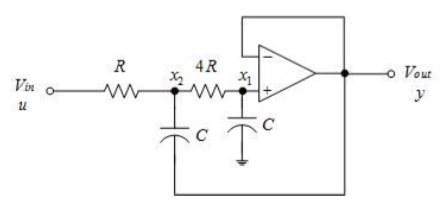
\includegraphics[width=0.6\linewidth]{circuit}
\caption{The circuit schematic for our plant. $C = 10\mu F$ and $R=50k\Omega$}
\label{fig:circuit}
\end{figure}

Immediately, we notice that $y=x_1$, because the $+$ and $-$ terminals of the op-amp must be at approximately equal potential.
This means that our output equation is:

\begin{equation}
y = \begin{bmatrix}
1 & 0
\end{bmatrix}
\begin{bmatrix}
x_1 \\ x_2
\end{bmatrix}
\end{equation}

We can use Kirchhoff's Current Law at the two nodes $x_1$ and $x_2$ to determine the rest of the state space equations for this system.

\begin{align}
x_1:&~~~~ \frac{1}{4R}(x_1-x_2) + C\dot{x}_1 = 0 \label{eq:KCL1} \\ 
x_2:&~~~~ \frac{1}{R}(x_2 - u) + \frac{1}{4R}(x_2-x_1) + C(\dot{x}_2-\dot{x}_1) = 0 \label{eq:KCL2}
\end{align}
%
Now if we solve equation \ref{eq:KCL1} for $\dot{x}_1$, we get:
\begin{equation}
\dot{x}_1 = \frac{1}{4RC}(-x_1+x_2)
\end{equation}
%
Solving equation \ref{eq:KCL2} for $\dot{x}_2$ (and plugging in the result above) we get:
%
\begin{equation}
\dot{x}_2 = \dot{x}_1+\frac{1}{4RC}(x_1-x_2)+\frac{1}{RC}(-x_2+u) =\frac{1}{RC}(-x_2+u)
\end{equation}
%
Putting these equations in matrix form, we obtain:
%
\begin{equation}
\begin{bmatrix}
\dot{x}_1 \\ \dot{x}_2
\end{bmatrix} = 
\begin{bmatrix}
\frac{1}{4RC} & -\frac{1}{4RC} \\
0    & -\frac{1}{RC}
\end{bmatrix}
\begin{bmatrix}
x_1 \\ x_2
\end{bmatrix} + 
\begin{bmatrix}
0 \\ \frac{1}{RC}
\end{bmatrix} u
\end{equation}
%
For our system, $\frac{1}{RC} = \frac{1}{50k\Omega*10\mu F} = 2\mathrm{Hz}$.
Using this, our equations become:
%
\begin{equation}
\begin{bmatrix}
\dot{x}_1 \\ \dot{x}_2
\end{bmatrix} = 
\begin{bmatrix}
\frac{1}{2} & -\frac{1}{2} \\
0    & -2
\end{bmatrix}
\begin{bmatrix}
x_1 \\ x_2
\end{bmatrix} + 
\begin{bmatrix}
0 \\ 2
\end{bmatrix} u
\end{equation}
\section*{Designing the Controller}
\subsection*{Discrete-Time Representation}
To design a digital control system, we need the equivalent discrete-time state space representation of the plant.
Matlab can generate this for us with the command {\tt c2d}.
The Matlab commands used to do this conversion and their outputs are included below:
\small
\begin{verbatim}
>> A = [-.5 .5; 0 -2]
>> B = [0; 2]
>> C = [1 0]
>> D = 0;
>> Ts = 0.1;
>> dt_sys = c2d(ss(A,B,C,D),Ts)

dt_sys =
 
  a = 
            x1       x2
   x1   0.9512  0.04417
   x2        0   0.8187
 
  b = 
             u1
   x1  0.004604
   x2    0.1813
 
  c = 
       x1  x2
   y1   1   0
 
  d = 
       u1
   y1   0
 
Sample time: 0.1 seconds
Discrete-time state-space model.
\end{verbatim}\normalsize
Using this, our discrete-time plant is:
\begin{align*}
\mathbf{x}[n+1] &= 
  \begin{bmatrix}
    0.951 & 0.0442\\
    0     & 0.819
  \end{bmatrix}
  \mathbf{x}[n] + 
  \begin{bmatrix}
    0.00460 \\ 0.181
  \end{bmatrix}u[n]\\
y[n] &= 
  \begin{bmatrix}
    1 & 0
  \end{bmatrix}
  \mathbf{x}[n]
\end{align*}

\subsection*{Full State Feedback}
Now that we have a discrete-time state space representation of our plant, we can design a full state feedback controller \emph{in discrete time} to control our system.

To do this, we will use optimal control and minimize the objective function 
\[
J = \frac{1}{2}\sum_{n=0}^{\infty}\left(20x_1[n]^2 + x_2[n]^2 +2u[n]^2 \right) 
\]
This is just a standard quadratic optimization of the form $J = \frac{1}{2}\sum\limits_{n=0}^{\infty}\left(\mathbf{x}[n]^T\mathbf{Qx}[n] + \mathbf{u}[n]^T\mathbf{Ru}[n] \right) $ where $\mathbf{Q} = \begin{bmatrix}20 & 0\\0 & 1\end{bmatrix}$ and $\mathbf{R} = 2$. 
We can use the Matlab command {\tt dlqr} to solve this optimization problem as follows:
\small
\begin{verbatim}
>> Ad = dt_sys.a;
>> Bd = dt_sys.b;
>> Q = [20 0; 0 1];
>> R = 2;
>> [K S P_K] = dlqr(Ad,Bd,Q,R)

K =

    1.6938    0.5148


S =

    142.8152   18.3179
    18.3179    6.1006


P_K =


    0.8344 + 0.0308i
    0.8344 - 0.0308i
\end{verbatim}\normalsize

From this output, we can see that our feedback gains are:
\[\mathbf{K} = \begin{bmatrix} 1.6938 & 0.5148\end{bmatrix}\]
And our system poles are:
\begin{align*}
z_1 &= 0.8344 + 0.0308i \\ z_2 &= 0.8344 - 0.0308i
\end{align*}

\subsection*{Observer}
In practice, we will not have direct access to the full state of our system.
Instead, we will need to approximate the state of the system with an observer of the form:

\begin{align*}
\hat{\mathbf{x}}[n+1] &= \mathbf{A}_d\hat{\mathbf{x}}[n]+ \mathbf{B}_d u[n] + \mathbf{L}(y[n]-\hat{y[n]} )\\
\hat{y}[n] &= \mathbf{C}\hat{\mathbf{x}}[n]
\end{align*}

Matlab can design this controller for us (by selecting {\bf L}) if we provide desired poles for the observer.
We need the observer to respond faster than the plant, so that we will be able to estimate the state of the system in real time.
To do this, we divide the values of the system poles by five to get the pole locations:

\begin{align*}
z_1 &= 0.1669 + 0.0062i \\ z_2 &= 0.1669 - 0.0062i
\end{align*}

Now, we can use Matlab to determine {\bf L}:
\small
\begin{verbatim}
>> P_L = P_K/5;
>> L = acker(Ad',C',P_L).'

L =

    1.4362
    9.6214
\end{verbatim}

Therefore, our observer gains are:
\[\mathbf{L} = 
    \begin{bmatrix}
       1.4362 \\
       9.6214
    \end{bmatrix}
\]

\subsection*{Reference Gain}
To have a usable system, we also need a reference gain $K_r$ that will be multiplied by the input.
We have the following formula for that reference gain in order to have zero steady-state error:
\[K_r = -\mathbf{\left[(C-DK)(A_\mathrm{d}-I-B_\mathrm{d}K)^\mathrm{-1}B_\mathrm{d}+D\right]}^{-1}\]
We can use Matlab to calculate this for us:
\small
\begin{verbatim}
>> I = eye(2);
>> Kr = -inv( (C-D*K)*inv(Ad-I-Bd*K)*Bd + D )

Kr =

    3.2086
\end{verbatim}
Therefore, our reference gain is:
\[K_r = 2.4140\]
\pagebreak\section*{Simulation}
To confirm that our design will meet the given specifications, we simulated the step response of the system in Simulink.
Our Simulink model is included as Figure \ref{fig:simulink}. \\

\begin{figure}[h]
\centering
    \begin{subfigure}[b]{0.65\textwidth}
        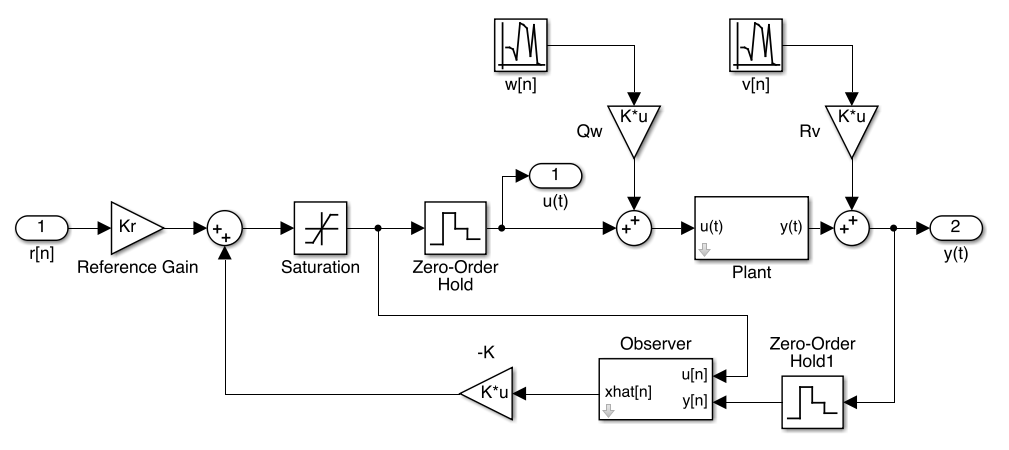
\includegraphics[width=0.9\textwidth]{system}
        \caption{The high level model for our control system}
        \label{fig:system}
    \end{subfigure}
    \\
    \begin{subfigure}[b]{0.35\textwidth}
        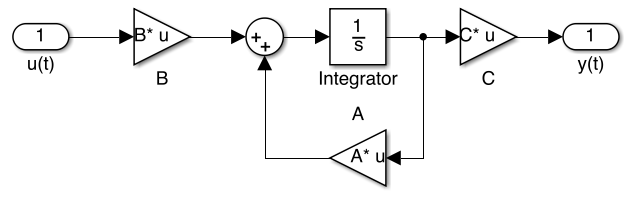
\includegraphics[width=0.9\textwidth]{plant}
        \caption{The model of our plant}
        \label{fig:plant}
    \end{subfigure}
    \begin{subfigure}[b]{0.35\textwidth}
        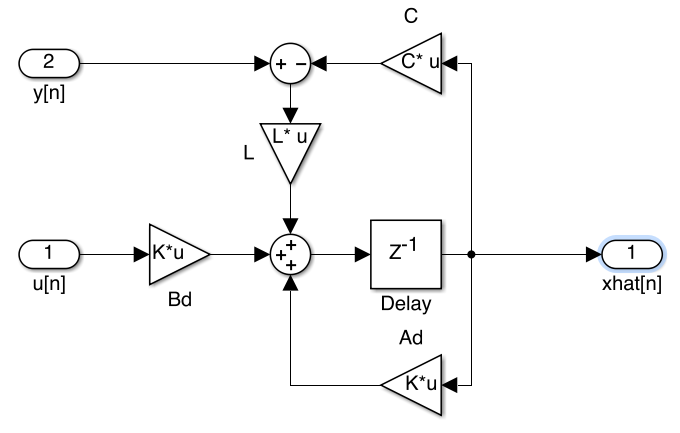
\includegraphics[width=0.9\textwidth]{observer}
        \caption{The model of our observer}
        \label{fig:observer}
    \end{subfigure}
    \caption{Our Simulink model}\label{fig:simulink}
\end{figure}

The results of the Simulation are summarized in Figure \ref{fig:sim_results}.
The system meets the given specifications of zero overshoot, zero steady state error, and a 2\% settling time under 4s.
The total control input is also relatively low, as desired.

\begin{figure}[h]
\centering
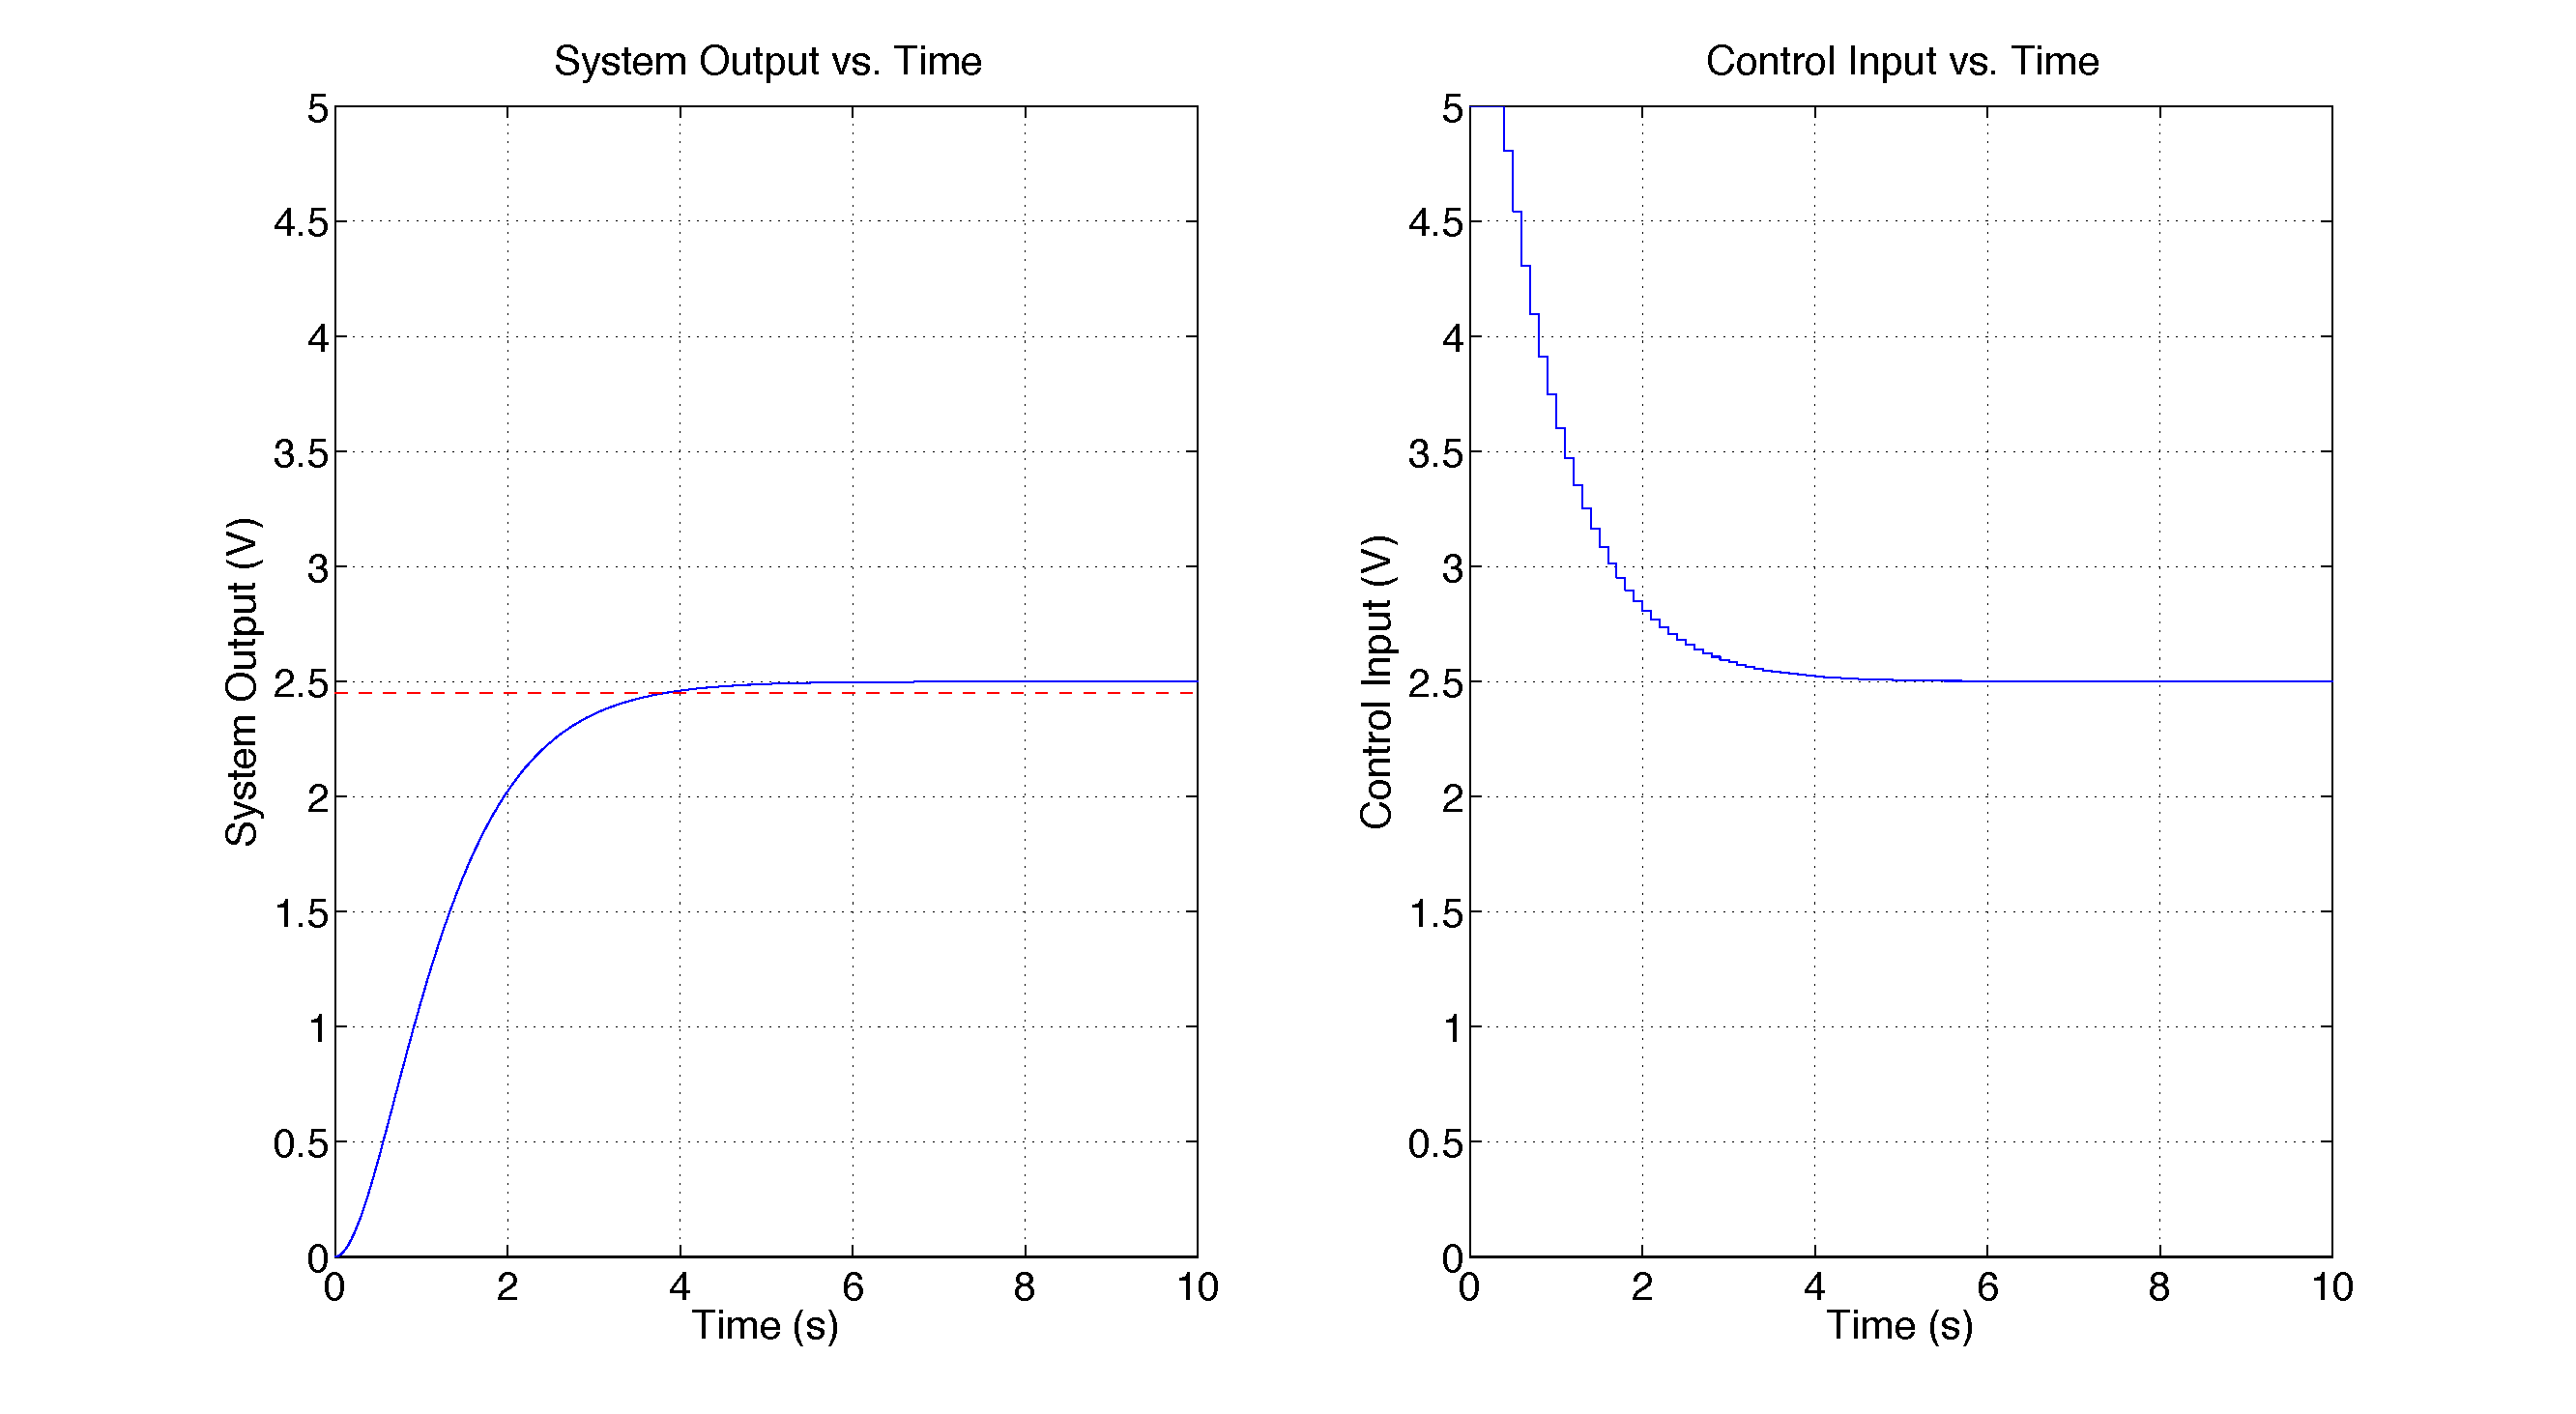
\includegraphics[width = 0.95\linewidth]{sim_results}
\caption{The results of our simulation}\label{fig:sim_results}
\end{figure}

\section*{Results}

We find that the actual system achieves a 2\% settling time under 4s, as desired.
Additionally, the system produces no overshoot and has zero steady state error.
The control input is saturated at the start of the step response as expected, because the error is large.
We found that our controlled system was slightly slower than the simulation, most likely due to parameter uncertainty in the resistors and capacitors. 

\begin{figure}[h]
\centering
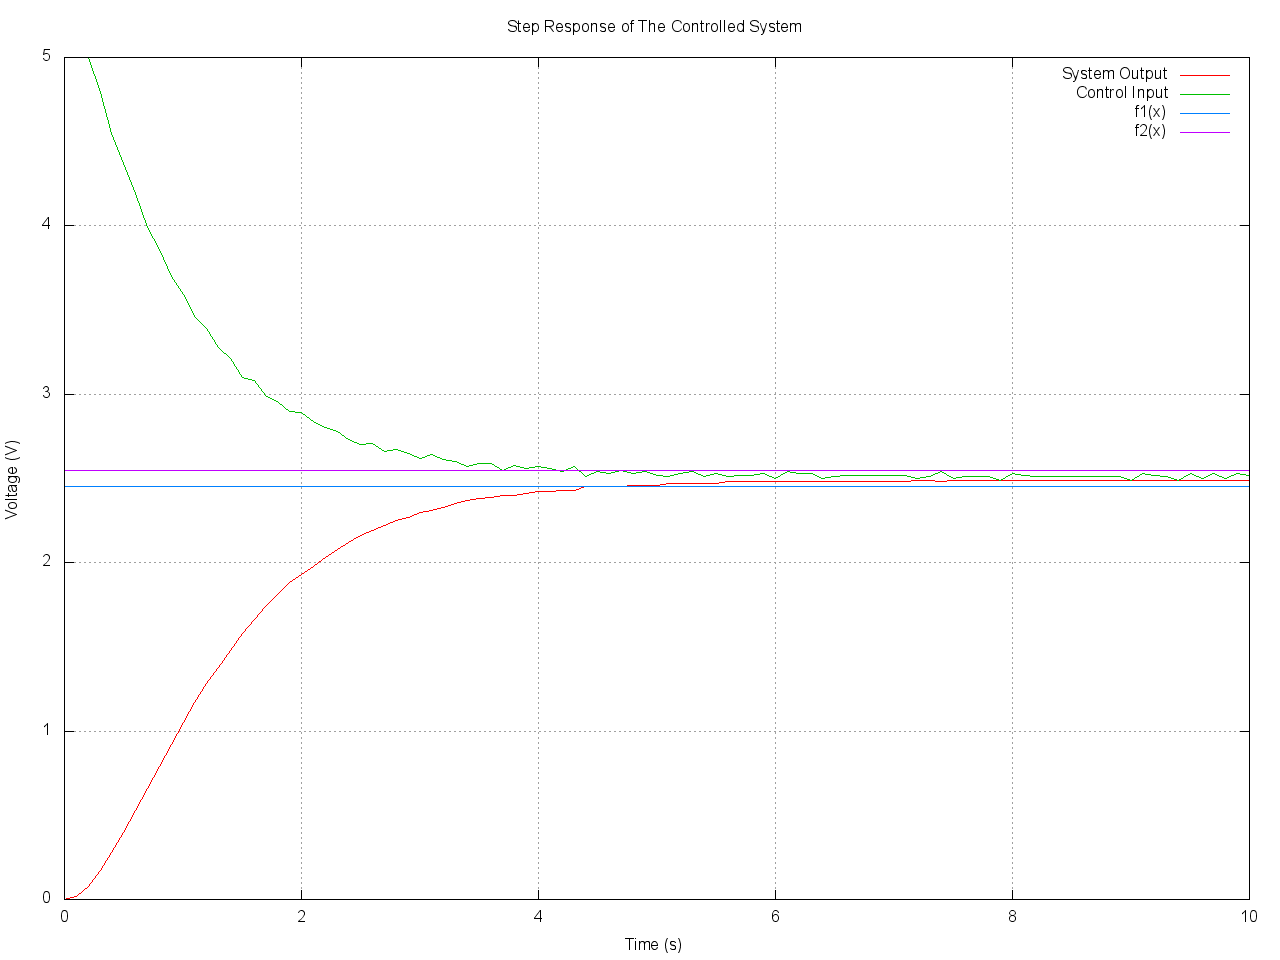
\includegraphics[width = 0.7\linewidth]{results}
\caption{The step response of our controlled system}\label{fig:results}
\end{figure}

\end{document}